Through the use of experimental results, we aim to prove several
claims made in this paper. First, we show that in some domains of
e-commerce measuring text diversity for product titles is a valid
approach for discovering interesetingness. To that end, we present the
unsupervised evaluation of diversity scores against human-made
interestingness labels for products in an eBay data-set of iPhone
cases. Second, we evaluate our proposed text diversity measure against
several baselines on the dataset based on NSF grant proposal
abstracts, to show that our model does in fact measure
diversity. Finally, as part of our model, we proposed a method for
extracting topic-distributional representations of words and
sentences. Even though it is not the main goal of the paper, we were
interested to see how these representations perform as feature vectors
in a supervised setting. To that end, we used the eBay product
dataset again, comparing against other text embedding techniques.

\subsection{Datasets}
\label{sec:datasets}


\begin{figure*}
\begin{center}
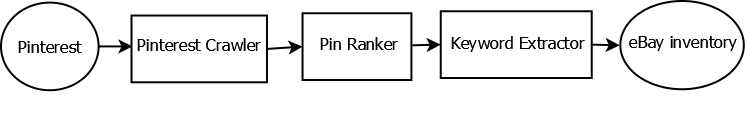
\includegraphics[height=2.5cm]{figures/Pipeline.png}
\caption{Pipeline for generating interesting eBay products based on Pinterest. Pinterest is first crawled, next the pins will be ranked and filtered based on whether or not they contain useful product information, next a product keyword extractor is applied to a set of highly ranked pins, and finally the extracted keywords are used to find a relevant eBay product.}
\end{center}
\label{fig:pinterest-pipeline}
\end{figure*}

We used the following two datasets in our experiments: 

{\bf Interesting iPhone cases}.
In this dataset, we generated a collection of interesting (positive) and uninteresting (negative) iPhone cases as follows. For generating positive examples, one natural choice was exploiting the data hosted by Pinterest. By definition, it is fair to assume that anyone who pins a product on Pinterest has found it interesting to some degree. The more a pin is engaged by the users, the more interesting is the product to those users. Although Pinterest data is biased by the demographic of its users, it is a publicly available dataset and is a more natural choice compared to collecting interesting products using crowd sourcing such as  {\em Amazon Mechanical Turk (AMT)} where it would be more subject to demographic biases. We built a pipeline for generating interesting eBay products illustrated in Figure~\ref{fig:pinterest-pipeline}.  In the first stage, we periodically crawl pins from Pinterest. In the next stage we filter the pins which do not have rich textual content and then rank the remaining pins using a score computed from the number of {\em repins}, {\em likes}, and {\em comments}. In the next stage, we trained a {\em Conditional Random Field (CRF)} model for extracting product related keywords from a set of highly ranked pins produced in the previous step. The final set of product related keywords  is then used to find a match in the eBay inventory. 

For generating the uninteresting iPhone case dataset (negative examples), we
hired workers from {\em AMT} to label a collection
of nearly 20,000 iPhone cases on {\em eBay}.  We then pulled our final dataset from the annotated by selecting only those instances where the annotators all labeled it as uninteresting. 

The final data-set consists of $2179$ positive and $9770$ negative instances
for a total of $11,949$ instances. For each instance, the product title of
the corresponding {\em eBay} listing was used as the input. In this case we are
dealing with very short text snippets, usually 10 to 12 words each. To
train a topic model, we used a larger, more broader set of about
$2$ million product titles, grouped based on {\em eBay} categorical information into about $8,000$
documents of approximately $200$ titles each. We used the Mallet LDA
implementation to learn a topic model with $400$ topics.


%{
% We used insights from 
% interesting iPhone cases found on {\em Pinterest} and {\em eBay's}
% user behavior data in order to generate a balanced data-set.  
% We then pulled our final dataset from the annotated by selecting only
% those instances where the annotators all labeled it as 
% positive (i.e., interesting) or negative (i.e., uninteresting). The
% final data-set consists of 2179 positive and 9770 negative instances
% for a total of 11,949 instances. For each instance, the product title of
% the corresponding {\em eBay} listing was used as the input. In this case we are
% dealing with very short text snippets, usually 10 to 12 words each. To
% train a topic model, we used a larger, more broader set of about
% 2 million product titles, grouped based on {\em eBay} categorical information into about 8,000
% documents of approximately 200 titles each.
%}

{\bf {\em NSF} abstracts}. For the second dataset we used a set of
61,902 National Science Foundation 
Scholarship proposal abstracts (see~\cite{bache:2013} for more
details) to evaluate how our diversity measure 
compares to other methods on larger pieces of text. We used this set
for training a topic model, however to get labeled data, we had to
generate artificial examples, by randomly mixing pairs of abstracts that we
could expect to be either similar (small diversity) or very different
(high diversity), based on the available meta-data, and labeling them accordingly. We generated 5,000 of
those examples with positive and negative labels evenly
represented. For this experiment, we trained a separate topic model with $300$ topics
based on the original NSF abstracts. To give better intuitions for
this setting, Table \ref{tab:nsf-examples} presents two example
abstracts - one, which the model deemed diverse, with score 1.25, and
a much less diverse one, with score 0.71. Note, that theoretically the
diversity may be anywhere between $0$ and $\log(|T|)\approx 5.7$, but
in practice, almost all of the documents fell into the range of $0.6$
to $1.3$. The table shows top three topics that the model associated
with each of the two example abstracts. For the more diverse abstract, the
topics (Linguistics, Design and Decision-Making) are relatively dissimilar,
while for the less diverse one (Algebraic Geometry, Combinatorics and
Foundations) they are closely related to each other, hence the lower score.  

\begin{table*}[t]
\renewcommand{\arraystretch}{1.3}
\caption{Examples of NSF Abstracts:
(left) example of an NSF proposal found by our approach to be more diverse (inter-disciplinary proposal); (right) example of an NSF proposal mostly centered on a single area.}
\label{tab:nsf-examples}
%\vspace{4mm}
\centering
\begin{tabular}{r|l|r|l}
\multicolumn{2}{c}{\bfseries High
  Diversity}&\multicolumn{2}{c}{\bfseries Low Diversity}\\
\hline\hline
\multicolumn{2}{c|}{{\bf Title}\hfill\quad {\em Linguistics-Based Preference Information Modeling for Design
Decision-Making}} & \multicolumn{2}{c}{{\bf Title}\hfill\quad {\em Ramsey Theory: Central sets and related
combinatorially rich sets}}\\
\hline
Main Topics & Top 5 words for topic & Main Topics & Top 5 words for topic\\
\hline
Linguistics & language, linguistic, english, speakers, words &
Algebraic Geometry& theory, algebraic, geometry, representation,
algebra\\
Design & design, engineering, principles, implementation,
methodology & Combinatorics & theory, graph, problems, discrete, combinatorial\\
Decision-Making &decision, making, uncertainty, risk, choice &
Foundations& theory, understanding, fundamental, framework, general
\end{tabular}
\end{table*}

% Three main topics: Language (138), Design (37), Decision-Making (208).

% Language (138): 1912        5659       11148       20337        4655        4784        5091        1044         334        6809
% language languages linguistic english speakers words word
% linguistics documentation translation
% Design (37):        212         162        5031        2667       1790        2781        1791         290         192        1489
% design engineering designs designing principles implementation
% methodology objective tools designers
% Proposal ? (253):         1105         291        5970        5414        5070        5674        3609       15718        2137        2508
% public award recovery act funded american law reinvestment employ
% funds 
% Decision-Making (208)        1063         875         898         874         449         788        3317        3569          32         792
% decision making decisions uncertainty risk make choice choices
% research individual

% Algebraic Geometry (41)          8         612          78         611         636      827         820        1347         829          12
% theory algebraic geometry representation algebra algebras quantum
% geometric mathematics study
% Combinatorics (28)           8        1683           7        1660         510        1338        1663          44          45         734
% theory graph problems graphs discrete combinatorial complexity
% applications areas set
% Theory (223)          8         914        2118          77         330         740         151        4049        1983         200
% theory theoretical theories understanding fundamental framework
% general string foundations ideas


% 0900255	07/01/2009	Division of Civil, Mechanical, and Manufacturing Innovation	ENGINEERING DESIGN AND INNOVAT; 	Linguistics-Based Preference Information Modeling for Design Decision-Making	This award is funded under the American Recovery and Reinvestment Act of 2009 (Public Law 111-5). The objective of this research award is to model the preference information embedded in natural language engineering design texts in order to identify linguistic forms of preference that will form the basis for a decision-making model that supports comparison of computed decisions to actual decisions. One view of the product design process is that it is driven by designers who have preferences for alternatives within a set of possible design choices. Such preference information is implicit within engineering design texts, but can be difficult to extract from unstructured information. The challenge is in linguistically modeling these preferences and mapping them into a mathematical model suitable for supporting design decision-making. Work will identify linguistic forms of preference, produce a comprehensive 'preference lexicon', develop formal mathematical models of preferences, and generate a decision-making model so that computed decisions can be compared with actual decisions to verify their validity.  If successful, this work will have impact across many industries, including product development, automotive, aerospace, and the military, due to the fundamental role of decision-making in the engineering design process. This research is intended to advance fundamental understanding of the language of design, in particular how preferences are expressed. In turn, this will further basic knowledge of the subjective aspects of decision-making and move towards the development of usable, effective decision support methods. The result will be an approach for imputing preference information as well as decision information from unstructured design texts that draws on both design language models and probabilistic extraction. Graduate students will learn about this work through an interdisciplinary, project-based class on decision-making in engineering design. A diverse group of undergraduates will have hands-on research experience with this work the Undergraduate Research Opportunities Program.


% 1160566	07/01/2012	Division of Mathematical Sciences	PROBABILITY; Combinatorics; 	Ramsey Theory: Central sets and related combinatorially rich sets	Ramsey Theory is that part of combinatorics that deals with the question of what sort of homogeneous structures one can expect to find in some one cell of a finite partition of a specified set (or sometimes in any suitably "large" subset). For example, the simplest nontrivial instance of the infinite version of Ramsey's Theorem says that whenever the two-element subsets of the set N of positive integers are finitely colored, there must be some infinite subset of N all of whose two element subsets are the same color. Many years ago, the principal investigator proved that whenever N is finitely colored, there must exist in one color an infinite sequence together with all of its finite sums of distinct terms without repetition. The original proof was elementary, but very complicated. Subsequently, other proofs were found that were less complicated. But in 1975, F. Galvin and S. Glazer showed that this "Finite Sums Theorem" is a completely trivial consequence of the fact that the Stone-Cech compactification of N can be given an algebraic structure extending ordinary addition which makes it a compact right topological semigroup, and therefore has idempotents. Sets with the property that they contain all the finite sums from a sequence are called IP sets. By virtue of the connection discovered above, a set is an IP set if and only if it has an idempotent in its closure in the Stone-Cech compactification of N. Those that have special idempotents which are called "minimal" in their closure are "central" sets. These sets have much stronger properties, many of which are consequences of the Central Sets Theorem. But central sets have a very complicated elementary description. Sets which satisfy the conclusion of the Central Sets Theorem are called "C-sets", and are much easier to describe in an elementary fashion. The proposed investigation of these various algebraically characterized large subsets of N should continue to yield new Ramsey-theoretic results.  A significant portion of the funds in this grant will provide support for graduate students at Howard University, an historically black university. In particular, the grant will provide stipends for three Ph.D. students, two of whom are black Americans, both female. This project will therefore be instrumental in training mathematicians who come from a population that is severely underrepresented within the population of US mathematicians.


\subsection{Unsupervised Setting}
\label{sec:unsupervised-learning}

We evaluated our text diversity model in an unsupervised learning task
on both datasets.
We implemented our model as described in
Sections~\ref{sec:information-diversity}-\ref{sec:topic-similarities} (labeled by {\em
    JSD-Sim-Con}) and compared it against a few 
baselines: Shannon entropy, Rao Diversity and a measure
based on Determinantal Point Processes.
The Shannon entropy has
been previously tested as a measure of document diversity with quite
underwhelming results in \cite{bache:2013}, where the authors proposed 
Rao diversity as a better solution, which incorporates the topic similarity
information to provide better accuracy. We suspected that
poor performance of entropy might be due to a suboptimal choice of
topic distribution, which led to our topic similarity
method. This technique can be used on any topic distribution
by simply multiplying it by the topic similarity matrix, and then
renormalizing. We present the performance of entropy with - and
without - the topic
similarity transformation to verify that this approach improves the results not
only for Jensen-Shannon Divergence, but for other measures as well.
Both for the entropy and Rao diversity, we generated topic
distributions by inferring them for each instance, based on the LDA
model, using the standard functionality from Mallet.

Determinantal Point Processes (DPP) have recently gained popularity as a
useful tool for sampling diverse subsets, with many applications
(see~\cite{kulesza:2012} for more details). We were interested to see
if they can also be useful for 
measuring the diversity of a set provided as input. Given a set of
instances described as feature vectors $U=\{v_i\}_{i=1}^N\subset \rr^T$, DPP defines a
sampling model for selecting a subset of $S=\{v_{i_j}\}_{j=1}^k$, by
setting the probability of $S$ proportional to the determinant of the
Gram matrix corresponding to those vectors. One might therefore
consider this determinant to be a good measure of set diversity,
because, intuitively, a more diverse set should have a higher
probability. The problem with this, however, is that determinants are
computationally unstable and very sensitive to local changes. For
example, if any two instances happen to have identical vector
representations, that immediately forces the determinant to $0$, even
though a set may be otherwise very diverse. We decided to use
another measure derived from a DPP. Instead of looking at a set $S$
(in our case, a set of words) as a sample from a larger set, we can
imagine sampling from $S$ itself. In that case, the average size of
the samples tells us how many significantly different words there are
in the given text. Fortunately, the expected sample size can be
computed from the eigenvalues of the aforementioned Gram matrix, as
discussed in \cite{kulesza:2012}. Two aspects of the feature
vectors are relevant for the DPP. The length of the vector represents
the relevance of the corresponding word, while the direction is
responsible for determining the pairwise similarities. For the
direction, we used the distributional representations from 
our model. For the vector lengths, we tried two versions: all
unit lengths (i.e. no preference), and using the importance values from
Definition \ref{mixture}. One drawback of the expected
DPP sample size is that it is correlated with the length of a
document. However, within each of our datasets, the instances have roughly
similar length.

Figures \ref{fig:roc-curves} (a) and (c)
present ROC curves comparing all of the diversity measures for each dataset.
In either case it can be observed
that our approach outperforms the other baselines, with an AUC
around $0.73$. Moreover, for the {\em eBay} dataset the other measures
give poor results. This can be explained as follows: since the
text snippets are short, the LDA may yield a poor topic inference for
such short text and as a result all measures using topic inference
would perform poorly. Our technique only relies on the topic model for
computing the distributional representations of words, so LDA can be
trained on a separate dataset and does not have to be affected by the
length of documents in the test set.
 The DPP-based measure does have some correlation
with the labels for both datasets, although not particularly
high. Interestingly, for the eBay dataset, unit vector lengths
performed better, while for NSF, importances gave an improvemet (in
each case, only the better result was
plotted). Another interesting observation is that 
Shannon entropy on the NSF dataset performs much better when applied
to distributions transformed using topic similarity information. In
fact, in our experiments it did better than Rao diversity, which also
used the same topic similarity matrix. This shows that the
transformation proposed in Section~\ref{sec:topic-similarities} is an
effective way of incorporating topic similarity information when
measuring diversity.
\begin{figure}
\begin{center}
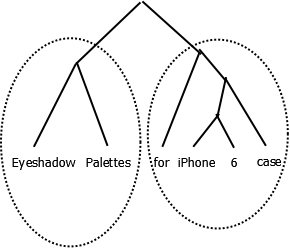
\includegraphics[width=5.5cm]{figures/RAE.png}
\caption{RAE tree learned for the product: {it Black Qi Standard Wireless Charging Charger Receiver Case For iPhone 5 5G}. Note how RAE learns to merge different concepts separately and merges them until very last step into the root node.}
\end{center}
\label{fig:rae-example}
\end{figure}

Figures~\ref{fig:roc-curves} (b) and (d)  
show the gains we obtain by applying topic
similarity and context conditioning techniques to our measure, as
discussed in Sections~\ref{sec:the-readers-model} and
\ref{sec:topic-similarities}. Both methods appear to be beneficial,
significantly improving the AUC. Interestingly, using
topic similarities appears to skew the ROC curve towards the upper
right, while context conditioning gives more improvement in the lower
left corner of the plot, which suggests that the two enhancements work
particularly well in conjunction. 
We also measured the difference between using 
the Informative Mixture and simply taking a uniform mixture of
distributional representations. The importances from
Definition~\ref{mixture} do not have much of an effect for the eBay
dataset, however they make a big difference
for the NSF proposal abstracts. This is probably because
the larger the size of the documents, the more important it is to
have an effective way of keeping all of the irrelevant words from
diluting the topic distribution. 

\begin{table*}[t]
\renewcommand{\arraystretch}{1.3}
\caption{Classification results for the eBay dataset.}
\label{tab:classification-results}
%\vspace{4mm}
\centering
\begin{tabular}{l||c|c|c|c}
&Precision & Recall & F1 & Accuracy
\\ \hline \hline
JSD Features         &$\mathbf{0.714}\pm 0.015$&$0.597\pm 0.016$&$0.650\pm
0.014$& $\mathbf{0.8828}\pm 0.0045$\\
RAE Features         &$0.676\pm 0.005$&$\mathbf{0.666}\pm 0.030$&$\mathbf{0.671}\pm
0.013$&$0.8809\pm 0.0020$ \\
SVD Features             &$0.676\pm 0.008$&$0.633\pm 0.017$&$0.654\pm
0.010$&$0.8778\pm 0.0027$\\
%\hline
\end{tabular}
\end{table*}

\subsection{Supervised Setting}
\label{sec:text-embeddings}

In the second set of results, we aim to show that topic-distributional
representations of words can be combined into useful feature vectors
for describing a block of text. Following the notation from
Definition~\ref{text-diversity}, let text $W$ be represented by 
$\cP_c=\{(\widehat{P}^{M_{\cP^i}}_{w_i},D_{w_i})\}_{i=1}^k$. We
describe $W$ with a feature vector defined as
\[F_{\cP_c}=\sum_{i=1}^k D_{w_i}\widehat{P}^{M_{\cP^i}}_{w_i}.\] Note, that this is identical to
the mixture distribution used in computing our text diversity measure, except
without the normalization factor, since it is not necessary in this setting.
We used those feature vectors in a supervised classification
task for the eBay dataset described in
Section~\ref{sec:datasets}. Specifically, in this setting, part of the labeled data
is used to train a classifier, which is given a feature vector
representation of a product title, and outputs an interestingness
label. We used two 
different feature-extraction techniques as baselines for
comparison. For the first baseline we used {\em Latent Semantic
  Indexing (LSI)} features by forming a 
document-term matrix and performing SVD. For the second baseline we used the {\em recursive auto-encoders (RAE)}~\cite{Socher:2011:SRA:2145432.2145450}. RAEs 
have been shown successful for sentence-level prediction of sentiment label
distributions. There is a nice connection between RAEs and text diversity: starting from the word level, an RAE greedily forms substructures that yield the least reconstruction error  structured in a  binary tree. As a result at the higher levels of the tree we observe the more diverse  substructures. This is further illustrated in Figure~\ref{fig:rae-example} where it shows the learned RAE structure for the example product shown in Table~\ref{tab:ebay-interesting-products}(a). When RAE is applied to the product title "Eyeshadow Palettes for iPhone 6 case" , we can observe that the words \{for, iPhone, 6, case\} are combined into one substructure, while the words \{Eyeshadow, Palettes\} form a different substructure. In other words RAEs inherently respect diversity at higher levels of the RAE tree structure.

Table~\ref{tab:classification-results} shows
the performance of the SVM classifier using our proposed mixture topic
distribution as features and compares it to these different baselines.
These results are averaged over five different cross-validation splits using $0.6$ for training
and $0.4$ for testing. Our proposed approach shows a higher precision
and a marginally higher accuracy compared to the baselines.
